%%%%%%%%%%%%%%%%
% Info on beamer: 
% 1) http://en.wikibooks.org/wiki/LaTeX/Presentations
% 2) Mertz2005
% 3) Rivero2012
%%%%%%%%%%%%%%%

%%%%%%%%%%%%%%%%%%%%%%%%%%%%%%%%
% this Latex template should be stored in: ~/Library/TeXShop/Templates
%%%%%%%%%%%%%%%%%%%%%%%%%%%%%%%%

\documentclass[xcolor=pdftex,dvipsnames,table, handout]{beamer}
% have a look at page 38 onwards of the documentation for the `xcolor` package in order to see predefined color names

%\hypersetup{pdfstartview={Fit}} % fits the presentation to the window when first displayed

% a couple of built-in themes
%\usetheme{Warsaw}
%\usetheme{Berkeley}
\usecolortheme{dolphin}

% suppress the navigation bar:
\beamertemplatenavigationsymbolsempty	

% packages:
\usepackage{booktabs} % for tables
\usepackage{natbib} % for citations
\usepackage{hyperref} % for hyperlinks
\usepackage{amssymb} % for mathematical symbols
\usepackage[overlay]{textpos}
%\usepackage{beamerthemesplit}
% others to try: beamerthemebars, beamerthemelined, beamerthemetree, beamerthemetreebars

% \usepackage{beamerthemesplit} // Activate for custom appearance

%%\usepackage[style=footnote-dw]{biblatex}
%% Package biblatex: '\bibliography' must be given in preamble.
%\usepackage[backend=biber,style=numeric-comp,sorting=none]{biblatex}
%\addbibresource{/Users/Claudius/Documents/MyLiterature/Literature.bib}
%%\bibliography{/User/Claudius/Documents/MyLiterature/Literature.bib}

% Note, paths need to end with a forward slash "/"
\graphicspath{
{/Users/Claudius/Documents/PhD/THESIS/kks32/LaTeX/2_Chapter/Figs/Raster/}
{/Users/Claudius/Documents/PhD/THESIS/kks32/LaTeX/Presentations/Group_meeting/figures/} 
{/Users/Claudius/Documents/PhD/THESIS/kks32/LaTeX/Data_analysis/reference-mapping/figure/}
{/Users/Claudius/Documents/PhD/PhDupgradeReport/}
{/Users/Claudius/Documents/PhD/Marie-Curie-ITN/Groningen09/ProjectPresentation/}
{/Users/Claudius/Documents/PhD/sRAD/sRAD_Analysis/}
{/Users/Claudius/Documents/PhD/THESIS/kks32/LaTeX/Presentations/PEB_Bialowieza/figures/}
{/Users/Claudius/Documents/PhD/THESIS/kks32/LaTeX/2_Chapter/figure/}
}

%-----------------------------------------

\title{Demographic history of a hybrid zone}
\subtitle{insights into the evolution of hybrid sterility \vskip80pt}
%\author{\vskip60pt \hskip-30pt \textcolor{BurntOrange}{Claudius Kerth\inst{1}} \vskip-10pt}
%\institute{
%\color{BurntOrange}
%\inst{1}
%Animal and Plant Science
%University of Sheffield, UK
%\vskip-10pt
%}
%\date{\color{BurntOrange} PEB Bia\l owieza, Sept, 2017}

\institute{
%vskip25pt
%\hskip25pt
\raggedright
{\hskip-3pt Claudius Kerth \& \\Roger Butlin}\\[5pt]
%	\inst{1}
	Animal and Plant Science\\[3pt]
	Sheffield University, UK\\[5pt]
%	Arthur Willis Environment Centre\\
%	\vskip15pt
%	\hskip4pt
	\textit{c.kerth@shef.ac.uk}
	\vskip10pt
}
\date{\scriptsize  PEB Bia\l owieza, 18 Sep 2017}


%%%%%%%%%%%%%
\begin{document}
%%%%%%%%%%%%%

%%%%%%%%%%%%%%%%%%%%%%%%
% Create Title page
%%%%%%%%%%%%%%%%%%%%%%%%
% Local background must be enclosed by curly braces for grouping.
{
\usebackgroundtemplate{\includegraphics[width=\paperwidth]{grasshopper}}%
\frame{
\titlepage	% this creates the title page with the info provided before the beginning of the document
}
}

%%%%%%%%%%%%%%%%%%%%%%%%
%--------------
\section{intro}
%--------------


\begin{frame}{Hybrid Zone in the Pyrenees}
\framesubtitle{between \textit{Chorthippus parallelus erythropus} and \textit{C. p. parallelus}}
\scriptsize
%\begin{center}
\begin{columns}
\column{0.5\textwidth}
\centering
\includegraphics[width=\textwidth]{PostGlacialExp}
\\postglacial range expansion from southern refugia
\column{0.5\textwidth}
\begin{itemize}
\item divergence in allopatry for $\sim$500,000 years with repeated secondary contacts during interglacial periods\smallskip
\item F1 male hybrids are almost completely sterile due to a disruption of the testes development\smallskip
\item no sterile males can be found in the hybrid zone\smallskip
\item some divergence in mating behaviour (song, cuticular hydrocarbons, female preference) but no signs of reinforcement\smallskip
\item subspecies host different strains of Wolbachia\smallskip
\item no significant differences in habitat between northern and southern edge of the hybrid zone $\rightarrow$ no locality dependent selection $\rightarrow$ \emph{tension zone}
\end{itemize}
\end{columns}
%\end{center}
\end{frame}

%\begin{frame}{Background}
%\includegraphics[width=\textwidth]{grasshopper}
%\end{frame}


%\begin{frame}{sterility}
%\scriptsize
%\begin{center}
%\begin{columns}
%\column[T]{.45\textwidth}
%\centering
%laboratory backcross
%\includegraphics[width=\textwidth]{BackcrossTestesDistr}\\
%\raggedleft\tiny{Llewellyn, A., PhD thesis, 2008}
%\vskip15pt
%\begin{itemize}
%\item 
%\end{itemize}
%\hskip10pt
%\pause
%\column[T]{.45\textwidth}
%\centering
%sterility cline
%\includegraphics[width=\textwidth]{sterility_cline}\\
%\raggedleft\tiny{Shuker et al., 2005}
%\vskip15pt
%\begin{itemize}
%\item sterility causing alleles are not fixed within pure populations of either subspecies
%\end{itemize}
%\end{columns}
%\end{center}
%\end{frame}
%
\begin{frame}{sample}
\begin{center}
\scriptsize
\includegraphics[width=.8\textwidth]{map-1_small}\\ \vskip5pt
18 male individuals from two pure populations of each subspecies
\begin{textblock}{10}(3, -11) \textit{parallelus}\end{textblock}
\begin{textblock}{10}(-2, -3) \textit{erythropus}\end{textblock}
\end{center}
\end{frame}
%

%--------------------------
\section{analysis pipeline}
%--------------------------

\begin{frame}{RAD de novo assembly}
\centering
\only<1-| handout:1->{
\includegraphics[height=.8\textheight]{DeNovoAssembly_sketch}}
%\pause
\only<2| handout:2>{\begin{textblock}{10}(2, -8) \includegraphics[width=.7\textwidth]{paired_end_assembly_sketch}\end{textblock}}
\only<4-| handout:3>{\begin{textblock}{10}(2, -9) \includegraphics[height=.3\textheight]{RADome}\end{textblock}}
%starcode, vsearch, rainbow, dDocent, Angsd, dadi, stairwayplot
\end{frame}
%
\begin{frame}{Filtering}
\begin{itemize}
\scriptsize
\baselineskip12pt
\item mismapping filter \\[10pt]
\item excessive coverage filter\\[10pt]
\item low complexity sequence filter (\texttt{dustmasker})\\[10pt]
\item minimum coverage filter (15 ind. with $\ge 3\times$ coverage)\\[10pt]
\item excess of heterozygotes filter
\end{itemize}
\end{frame}
%
\begin{frame}{filtering for deviation from HWE}
\centering
\includegraphics[width=0.9\textwidth]{MAF_by_pval_ery}
\end{frame}
%
\begin{frame}{\texttt{ANGSD}}
\framesubtitle{population genetics with genotype likelihoods}
\scriptsize
\begin{description}
\scriptsize
\item[genotype likelihood] probability of the sequencing data given a genotype for a particular individual and particular site (up to a scaling factor)\\[5pt]
\end{description}
\vskip10pt
\begin{itemize}
\item no SNP nor genotype calling required\pause
\item allows for many population genetic analyses in a probabilistic framework, i. e. incorporating uncertainty in SNP's or genotypes, e. g.:
\begin{itemize}
\scriptsize
\item admixture analysis
\item inbreeding coefficients (e. g. $F_{ST}$)
\item association studies
\item site frequency spectrum (SFS) based analyses
\end{itemize}
\pause
\vskip5pt
\item allows utilisation of low-coverage sequencing data ($\le 10\times$) and maximisation of sample size to increase power of analyses\\[5pt]\pause
\item no hard filtering of SNP's or genotypes based on uncertainty that otherwise discards valuable information 
\end{itemize}
\vskip20pt
\raggedleft cf. \cite{Li2011, Nielsen2012}
\end{frame}
%
\begin{frame}{removing PCR duplicates}
\centering
\begin{columns}
\column{.5\textwidth}
\includegraphics[width=\textwidth]{ind-cov-dist-1}
\column{.5\textwidth}
\includegraphics[width=\textwidth]{dedup}
\end{columns}
\end{frame}

%--------------------------
\section{results}
%--------------------------

\begin{frame}{genetic differentiation}
\includegraphics[width=.5\textwidth]{PCA-1}
\includegraphics[width=.5\textwidth]{permut-global-fst-hist-1}
\end{frame}

\begin{frame}{folded minor allele frequency spectrum (SFS)}
\scriptsize
\centering
\begin{columns}
\column{.5\textwidth}
\begin{figure}
\includegraphics[width=\textwidth]{folded-sfs-boot-1}
\begin{textblock}{6}(0, -6.5)\raggedleft\tiny $\sim$36,850 SNP's\end{textblock}
\begin{textblock}{6}(0, -5.5)\raggedleft\tiny Tajima's D: -0.345\end{textblock}
\end{figure}
\column{.5\textwidth}
\begin{figure}
\includegraphics[width=\textwidth]{folded-sfs-boot-2}
\begin{textblock}{6}(0, -6.5)\raggedleft\tiny $\sim$49,968 SNP's\end{textblock}
\begin{textblock}{6}(0, -5.5)\raggedleft\tiny Tajima's D: -0.936\end{textblock}
\end{figure}
\end{columns}
\vskip15pt
from 1,130,775 sites on 22,742 contigs
\end{frame}
%
\begin{frame}{\texttt{stairway-plot}}
%\centering
\includegraphics[width=.9\textwidth]{PAR_-_200_bootstrap_replicates_final_summary}
\begin{textblock}{10}(12, -3.5) PAR\end{textblock}
\vskip10pt
\includegraphics[width=.9\textwidth]{ERY_-_200_bootstrap_replicates_final_summary}
\begin{textblock}{10}(12, -4) ERY\end{textblock}

%\begin{itemize}
%\item PAR ancient population size much greater than ERY
%\item evidence for a recent bottleneck in PAR and ERY
%\end{itemize}
\end{frame}
%
\begin{frame}{folded joint minor allele frequency spectrum (2D SFS) }
\begin{figure}
\includegraphics[width=\textwidth]{2DSFS_folded}
\begin{textblock}{8}(-1, -12)\raggedleft\tiny $\sim$74,058 SNP's\end{textblock}
%\begin{textblock}{6}(0, -5.5)\raggedleft\tiny Tajima's D: -0.345\end{textblock}
\end{figure}
\end{frame}
%
\begin{frame}{varying divergence time or migration rate}
\begin{columns}
\column{.55\textwidth}
\centering\scriptsize
\begin{figure}
\includegraphics[width=\textwidth]{divergence_time_series}
\begin{textblock}{6}(0.5, -12.5)\centering\tiny increasing divergence time\vskip-5pt\end{textblock}
\end{figure}
\column{.55\textwidth}
\centering\scriptsize
\begin{figure}
\includegraphics[width=\textwidth]{migration_rate_series}
\begin{textblock}{6}(0.5, -12.5)\centering\tiny increasing migration rate\vskip-5pt\end{textblock}
\end{figure}
\end{columns}
\end{frame}
%
\begin{frame}{\texttt{$\delta$a$\delta$i}}
\framesubtitle{two epoch model}
\centering
\includegraphics[height=.8\textheight]{two_epoch_combined}
\begin{textblock}{6}(9, -8)\scriptsize -logL 21,009\end{textblock}
\end{frame}
%
\begin{frame}{\texttt{$\delta$a$\delta$i}}
\framesubtitle{primary contact model}
\includegraphics[height=.5\textheight]{ancient_migration_edited}
\begin{textblock}{6}(11, -5)\scriptsize  -logL 21,301\end{textblock}
%\begin{itemize}
%\item show graphics of models
%\item evidence for recent bottleneck in PAR, but much weaker in ERY
%\item can the level of gene flow be considered low?
%\item much greater gene flow from PAR into ERY
%\end{itemize}
\end{frame}
%

% --------------------
\section{summary}
% --------------------

\begin{frame}{summary}
\begin{itemize}
\scriptsize
\item no divergence in allopatry\\[10pt]\pause
\item allowing for gene flow doubles the estimated divergence time (0.5 $\rightarrow$ 1.1 mya)\\[10pt]\pause
\item gene flow had been about 5 times higher in the direction from PAR $\rightarrow$ ERY than vice versa\\[10pt]\pause
\item gene flow was low enough to allow divergence by drift (not just due to divergent selection pressures), see \citealt{Bank2012a}\\[10pt]\pause
%\item there is no clear signal of a recent population size increase in either subspecies (apart from negative Tajima's D), as would be expected from the range expansion after the last ice age ($\sim$8-6 kya)\pause
\item the PAR population had a greater ancient population size than ERY\\[10pt]\pause
\item there seems to be a signal of a recent drastic bottleneck at least in PAR (the signal for ERY is more ambiguous) as expected from serial founder events during range expansion\\[10pt]\pause
\item primary contact (ancient gene flow) fits the data better than secondary contact model $\Rightarrow$ no significant signal of recent gene flow (not enough power?)\\[10pt]\pause
\end{itemize}
\end{frame}
%



\begin{frame}{coalescent simulations}
\framesubtitle{from best fitting demographic models}
\centering
work in progress, sorry!
\end{frame}
%

\begin{frame}[allowframebreaks] % the option "allowframebreaks" is very handy for spreading content over several slides
\frametitle{For Further Reading}
\scriptsize
\bibliographystyle{elsarticle-harv}
\bibliography{/Users/Claudius/Documents/MyLiterature/Literature}
\end{frame}

\begin{frame}{Thanks to \ldots}
\centering

\includegraphics[height=.8\textheight]{Thanks_to}
\end{frame}

%--------------
\end{document}
%--------------

%----------------------------------------------------------------------

\begin{frame}{each restriction site produces two tightly linked RAD tags}
\begin{center}
\begin{description}
\footnotesize
\item[RAD tag] marker locus; one of the sequences upstream or downstream of the restriction site
\end{description}
\vskip15pt
\includegraphics[height=.6\textheight]{RADprocessoverview}
\begin{block}{}
\centering
\scriptsize
reduced representation of the genome results in higher read coverage as compared to whole genome sequencing given the same amount of sequencing effort
\end{block}
\end{center}
\end{frame}

%--------------
%\end{document}
%--------------

\begin{frame}{each restriction site produces two tightly linked RAD tags}
\begin{center}
\begin{description}
\footnotesize
\item[RAD tag] marker locus; one of the sequences upstream or downstream of the restriction site
\end{description}
\vskip15pt
\includegraphics[height=.6\textheight]{RADprocessoverview}
\begin{block}{}
\centering
\scriptsize
reduced representation of the genome results in higher read coverage as compared to whole genome sequencing given the same amount of sequencing effort
\end{block}
\end{center}
\end{frame}
%
%
%
\begin{frame}[label=sRAD]{RAD \`a la \cite{Baird2008}}
\centering
\begin{columns}
\column{.6\textwidth}
\uncover<1->{\includegraphics[width=\textwidth]{RADprotocolOverview_1}}
\uncover<2->{\includegraphics[width=\textwidth]{RADprotocolOverview_2}}
\uncover<3->{\includegraphics[width=\textwidth]{RADprotocolOverview_3}}
\column{.5\textwidth}
\begin{itemize}[<+->]
\scriptsize
\item<1-> one restriction enzyme \smallskip
\item<1-> pooling of samples after ligation of first adapter \smallskip
\item<1-> random shearing of fragments before gel size selection \\
\includegraphics[width=.3\textwidth]{SizeSelection_180610} \smallskip
\item<2-> selective PCR after ligation of second adapter \smallskip
\item<2-> only fragments with at least one P1 adapter get amplified \smallskip
\item<3-> paired-end contig can be assembled for blasting
\end{itemize}
\end{columns}
\end{frame}

\begin{frame}{the fundamental problem}
\framesubtitle{dominance of singleton loci in the \texttt{stacks} assembly}
\vskip25pt
\begin{columns}
\column{.5\textwidth}
\includegraphics[width=\textwidth]{dist_geno_calls}
\column{.5\textwidth}
\includegraphics[width=\textwidth]{MiSeq_dist_of_cov}
\end{columns}
\vskip25pt
\begin{block}{}
\centering
What could be the reason for this result?
\end{block}
\end{frame}

\begin{frame}{a strange observation}
\centering
\footnotesize
0.034\% of quality filtered reads contain an SbfI recognition site
\vskip15pt
\begin{columns}
\column{.5\textwidth}
\includegraphics[width=\textwidth]{SbfI_positions_in_uniqued__by_ind___reads-1}
\column{.5\textwidth}
\includegraphics[width=1.1\textwidth]{SbfI_frequency_dist__per_ind_-1}
\end{columns}
\medskip
\pause
\begin{block}{}
\centering
Could this indicate incomplete digestion?
\pause
$\Rightarrow$ could be tested with PCR over restriction sites
but no reference sequence to design PCR primers
\end{block}
\end{frame}

\begin{frame}[shrink]
\frametitle{a locust transcriptome as reference}
\medskip
\scriptsize
from the migratory locust \textit{Schistocerca gregaria}
\medskip
\begin{center}
\includegraphics[width=.8\textwidth]{igv_LC_1628_C1_Contig1776_standRAD}
\end{center}
\pause
\begin{description}
\scriptsize
\item[linked RAD tag site] detected if there is at least one "properly mapped" read pair on either side of an SbfI restriction site
\end{description}
\pause
collect all paired-end reads whose single-end mate mapped to a detected \textrm{linked RAD tag} site
$\Rightarrow$ assembly into contigs
\end{frame}

\begin{frame}{}
\begin{itemize}
\item detected 77 \textit{Schistocerca} reference contigs with linked RAD tags site \pause \vskip10pt
\item chose assembler programme \texttt{SSAKE} because it can be set to allow low coverage for contig extension \pause \vskip10pt
\item \texttt{SSAKEoptimiser.pl} to find optimal kmer length for each individual assembly, optimisation for length of longest contig assembled \pause \vskip10pt
\item 64 \textit{Schistocerca} reference contigs with a RADtag site for which at least one upstream and one downstream \texttt{SSAKE} contig could be assembled
\end{itemize}
\end{frame}

\begin{frame}{parallelising the search for the optimal kmer length}
\begin{center}
\vskip -20pt
\includegraphics[width=.8\textwidth]{SSAKEoptimiser_runtimes}
\end{center}
\end{frame}

\begin{frame}{manual merging of \texttt{SSAKE} contigs}
variation in input sequences interferes with contig assembly\\ \vskip 15pt
\begin{center}
\includegraphics[width=\textwidth]{contig_alignment}
\end{center}
\end{frame}

\begin{frame}{picking the right \texttt{SSAKE} contig}
\footnotesize
\texttt{SSAKE} generally assembles many contigs for a given set of sequences\\ \vskip15pt
\texttt{blast} of \texttt{SSAKE} contigs against their putative \textit{Schistocerca} reference contig\\ \vskip15pt
\begin{center}
\includegraphics[width=.9\textwidth]{SSAKE_contigs_aligned_against_Schisto_contig}
\end{center}
check that the assembled upstream and downstream \texttt{SSAKE} contigs actually belong to the same locus, i. e. RADtag site
\end{frame}

\begin{frame}
\footnotesize
\begin{itemize}
\item for 20 \texttt{Schistocerca} cDNA contigs I could assemble and confidently pick down and upstream contigs for PCR primer design \pause
\item backmapping of reads against this new small reference made up of pairs of PE contigs $\Rightarrow$ \textrm{targeted alignment} \pause
\begin{center}
\includegraphics[width=\textwidth]{stampy_par_34-10_vs_primer3ready_igv}
\end{center} 
\pause
\item \texttt{Coval-refine}
\end{itemize}
\end{frame}

\begin{frame}{Coval-refine}
\begin{columns}
\column{.1\textwidth}
after
\vskip50pt
before
\column{.9\textwidth}
\includegraphics[width=\textwidth]{stampy_par_34-10_vs_primer3ready_after_coval-refine_igv}
\end{columns}
\end{frame}

\begin{frame}{Backmapping results}
\begin{columns}
\column{.6\textwidth}
\begin{center}
\includegraphics[width=\textwidth]{fragments_mapped_per_ind-1}
\end{center}
\pause
\column{.4\textwidth}
rather even fragment number from all individuals \\
$\Rightarrow$ incomplete digestion is unlikely to be the reason for the dominance of singleton loci in the \texttt{stacks} assembly
\end{columns}
\begin{description}
\vskip15pt
\centering
\scriptsize
\item [fragment] non-PCR duplicate
\end{description}
\end{frame}


\begin{frame}
\centering
\footnotesize
Does the number of reads mapped back from an individual to the PE contig reference correlate with the total read number of reads from that individual?
\vskip20pt
\begin{columns}
\column{.5\textwidth}
\includegraphics[width=\textwidth]{frag_input_corr_fig-1}
\column{.5\textwidth}
\includegraphics[width=\textwidth]{frag_input_corr_fig-2}
\end{columns}
\vskip20pt
\end{frame}

\begin{frame}
%\centering
\footnotesize
Could this problem be alleviated with sequencing more reads from the same library? 
\begin{center}
%\includegraphics[width=0.7\textwidth]{PCR_duplicates}
\end{center}
\vskip10pt
Or, could low PCR template amount explain dominance of singleton loci in RAD tag assembly?
\end{frame}

\begin{frame}
\footnotesize
{\color{RoyalBlue!80}{If I added 100 ng of grasshopper DNA to the PCR mix, assuming that the genome is 12 Gbp long, this would only correspond to 7604 template molecules for the primers.}}
\vskip20pt
\begin{align}
\text{molar amount of template} &= \frac{\text{amount of DNA}}{\text{MW of bp} \times \text{genome size}} \nonumber \\[10pt]
&= \frac{100 \times 10^{-9}g}{660 \frac{g}{mol \times bp} \times 12 \times 10^{9} \text{bp}} \nonumber \\[10pt]
&= 1.26 \times 10^{-20} \text{mol} \nonumber
\end{align}
\begin{align}
\text{number of template molecules} &= 1.26 \times 10^{-20} \text{mol} \times \text{Avogadro's number} \nonumber \\[10pt]
&= 1.26 \times 10^{-20} \text{mol} \times 6.0221413 \times 10^{23} \nonumber \\
&= 7604 \nonumber
\end{align}
\end{frame}

\begin{frame}
\centering
SbfI sites in reads due to fragment-to-fragment re-ligation?
\end{frame}


%------------------------------------------------------------------------------------------

\begin{frame}[allowframebreaks] % the option "allowframebreaks" is very handy for spreading content over several slides
\frametitle{For Further Reading}
\scriptsize
\bibliographystyle{elsarticle-harv}
\bibliography{/Users/Claudius/Documents/MyLiterature/Literature}
\end{frame}


%------------------------------------------------------------------------------------------
% Example Slides and showcases
%------------------------------------------------------------------------------------------

%%%%%%%%%%%%%%%%%%%%%%%%%%%%%
%% overlays
%%%%%%%%%%%%%%%%%%%%%%%%%%%%%
%\frame
%{
%  \frametitle{Features of the Beamer Class}
%%  \framesubtitle{}
%  \begin{itemize}
%  \item<1-> Normal LaTeX class.
%  \item<2-> Easy overlays.
%  \item<3-> No external programs needed.      
%  \end{itemize}
%}
%%%%%%%%%%%%%%%%%%%%%%%%%%%%%

%%%%%%%%%%%%%%%%%%%%%%%%%%%%%
%% examples of `block` types
%%%%%%%%%%%%%%%%%
%\begin{frame}{Block types}
% 
%   \begin{block}{This is a Block}
%      This is important information
%   \end{block}
%
% 	\vskip20pt
%
%   \begin{alertblock}{This is an Alert block}
%   This is an important alert
%   \end{alertblock}
% 
%   \begin{exampleblock}{This is an Example block}
%   This is an example 
%   \end{exampleblock}
% 
%\end{frame}
%%%%%%%%%%%%%%%%%%%%%%%%%%%%%

%%%%%%%%%%%%%%%%%%%%%%%%%%%%%
% dividing the slide into columns
%%%%%%%%%%%%%%%%%%%%%%%%%%%%%%
%\begin{frame} 
%\frametitle{Two Column Output}
%\begin{columns}[c] 
%\column{.5\textwidth} 
%Practical \TeX\ 2005\\
% \vskip20pt
%Practical \TeX\ 2005\\ 
%Practical \TeX\ 2005
%\column{.5\textwidth} 
%\includegraphics[width=\textwidth]{/Users/Claudius/Documents/PhD/Presentations/journal_club/Orozco2012/PNG/isofemale_line.pdf}
%\end{columns}
%\end{frame}
%%%%%%%%%%%%%%%%%%%%%%%%%%%%%

%%%%%%%%%%%%%%%%%%%%%%%%%%%%%
% Definitions:
%%%%%%%%%%%%%%%%%%%%%%%%%%%%%%
%\frame{
%\frametitle{how to give a definition of a word}
%\begin{description}
%\item[isofemale line] a line started from a single mated female
%\end{description}
%}
%%%%%%%%%%%%%%%%%%%%%%%%%%%%%

%%%%%%%%%%%%%%%%%%%%%%%%%%%%%
% % table with row colors
%%%%%%%%%%%%%%%%
%\begin{frame}[fragile]
%testcolors
%\frametitle{A table with alternating row colors}
%\small
%In order for this to work, call the \textrm{beamer} class with the following options:
%\begin{verbatim}
%\documentclass[xcolor=pdftex, dvipsnames, table]{beamer}
%\end{verbatim}
%\vskip20pt
%\begin{center}
%\rowcolors{1}{RoyalBlue!20}{RoyalBlue!5} % these are `dvipsnames` from the xcolor package
%\begin{tabular}{lccr}
%\toprule
%This & is & the & header \\ [5pt]
%\midrule
%This & is the & content of & the first line \\
%This & is the & content of & the second line \\
%\bottomrule
%\end{tabular}
%\end{center}
%\vskip20pt
%The \colorbox{yellow}{rowcolors} command has to come right before the \textrm{tabular} environment.
%% The `rowcolors` command is provided by the `xcolor` package.
%\end{frame}
%%%%%%%%%%%%%%%%%%%%%%%%%%%%%

%%%%%%%%%%%%%%%%%%%%%%%%%%%%%
% overlays with \pause
%%%%%%%%%%%%%%%%%
%\begin{frame}[fragile] % the fragile option to the frame command is necessary if you want to use `verbatim` environments.
%\frametitle{Overlays with {\tt pause}}
%
%\setbeamercovered{dynamic}
%% overlays not yet revealed will faintly appear. Use "invisible" to turn that off.
%The command:
%\begin{verbatim}
%\setbeamercovered{dynamic} 
%\end{verbatim}
%\ldots allows overlays not yet revealed to be already faintly appear.
%\vskip20pt
%Practical \TeX\ 2005\\ \pause 
%Practical \TeX\ 2005\\ \pause 
%Practical \TeX\ 2005 
%\\ this does also work for graphics? \\ 
%\end{frame}
%%%%%%%%%%%%%%%%%%%%%%%%%%%%%

%%%%%%%%%%%%%%%%%%%%%%%%%%%%%
%%
%%%%%%%%%%%%%%%%%%%%%%%%%%%%%
%\begin{frame}[fragile] 
%\frametitle{Tic-Tac-Toe via {\tt tabular} and \textrm{onslide}}
%Overlays that are not yet revealed can be made invisible by this command:
%\begin{verbatim}
%\setbeamercovered{invisible} 
%\end{verbatim}
%\vskip20pt
%{\Huge 
%\begin{center}
%\begin{tabular}{c|c|c} 
%\onslide<9->{O} & \onslide<8->{X} & \onslide<2->{X} \\ 
%\hline \onslide<6->{X} & \onslide<3->{O} & \onslide<5->{O} \\ 
%\hline \onslide<10->{X} & \onslide<7->{O} & \onslide<4->{X}
%\end{tabular} 
%\end{center} 
%} 
%\end{frame}
%%%%%%%%%%%%%%%%%%%%%%%%%%%%%

%%%%%%%%%%%%%%%%%%%%%%%%%%%%%%%
% a slide with references
%%%%%%%%%%%%
%Citations used on the previous slides should appear here.
%\begin{frame}[allowframebreaks] % the option "allowframebreaks" is very handy for spreading content over several slides
%\frametitle{For Further Reading}
%\scriptsize
%\bibliographystyle{elsarticle-harv}
%\bibliography{/Users/Claudius/Documents/MyLiterature/Literature}
%\end{frame}
%%%%%%%%%%%%%%%%%%%%%%%%%%%%%%%



%%		%%
%		
%
%
%
%
%%		%%


%%%%%%%%%%%%%%%%%%%%%%%%%%%
%% simple list with overlays and hyperlink
%%%%%%%%%%%%%%%%%%%%%%%%%%%
%\frame{
%\frametitle{Santa Rosalia}
%\begin{itemize}
%\item Why are there so many species on earth? \pause
%\vskip10pt
%\item Why aren't there even more? \pause
%\vskip10pt
%\item Ecological constraints to diversity? 
%	\begin{itemize}
%	\item competition between species ?
%	\item Can we expect lots of ecologically identical species ? 
%	\\ $\rightarrow$ \href{http://www.nature.com/scitable/knowledge/library/neutral-theory-of-species-diversity-13259703}{\color{RoyalBlue!80}{neutral theory of species diversity}} \pause
%	\end{itemize}
%\vskip10pt
%\item Evolutionary constraints to diversity? 
%	\begin{itemize}
%	\item additive genetic variation ?
%	\item gene flow ?
%	\item recombination ?
%	\item lack of recombination ?
%	\end{itemize}
%\end{itemize}
%}
%%%%%%%%%%%%%%%%%%%%%%%%%%%



%%%%%%%%%%%%%%%%%%%%%%%%%%%%%%%%%%%%%%%%%%%%
% frame subtitle
% quotation
% item list with custom item symbols
% subdivision with columns
% including a figure
% font size
% inserting custom space
%%%%%%%%%%%%%%%%%%%%%%%%%%%%%%%%%%%%%%%%%%%%
% in order to use pictures from papers: grab them with the `Grab` app and use the `ConvertToPNG` AppleScript to convert them to .png format. 
% The output of the script is in a folder called `PNG` on the desktop.
%\begin{frame}%[allowframebreaks]
%\frametitle{The haploid model}
%\framesubtitle{local adaptation --  postzygotic isolation}
%
%\footnotesize
%
%\vskip5pt
%
%\begin{quote}
%\ldots it is the simplest model I can find which exhibits many of the genetic effects which will be found in more complex, more realistic models of speciation.
%\end{quote}
%\begin{itemize}
%\item infinite$^{1}$ haploid$^{2}$ population with discrete$^{3}$ generations, i. e.
%	\begin{itemize}
%	\item [1] no genetic drift
%	\item [2] no heterozygous effects
%	\item [3] non-overlapping generations
%	\end{itemize}
%\item two loci for local adaptation --  B/b and C/c
%\end{itemize}
%
%\pause
%\vskip10pt
%
%\begin{columns}
%\column{.5\textwidth}
%%\includegraphics[width=\textwidth]{fig_1}
%\column{.5\textwidth}
%\begin{itemize}
%\item multiplicative combination of fitness effects across loci
%\item average fitness across habitats of genotypes \textit{BC} and \textit{bc} always greater than their recombinants
%\end{itemize}
%\end{columns}
%
%\end{frame}
%%%%%%%%%%%%%%%%%%%%%%%%%%%%%%%%%%%%%%%%%%%%%%%%%%%%



%%%%%%%%%%%%%%%%%%%%%%%%%%%%%%
% using the `shrink` option to the frame command 
% to allow more content to fit on the slide
%%%%%%%%%%%%%%%%%%%%%%%%%%%%%%
%\begin{frame}[shrink]
%\frametitle{The haploid model}
%\framesubtitle{assortative mating -- prezygotic isolation}
%
%\begin{itemize}
%\item assortative mating locus A/a
%\item $d$ is the proportion of individuals which mate positive assortatively, i. e. strength of assortative mating
%\end{itemize}
%
%\begin{center}
%%\includegraphics[width=.6\textwidth]{fig_2}
%\end{center}
%
%\begin{quote}
%The A locus controls the division of the mating pool into two mating groups according to space, time or phenotype. 
%\end{quote}
%
%\color{red}{Find biological examples for assortative mating according to \emph{space}, \emph{time} or \emph{phenoptype} directed by alleles at a \underline{single} locus!}
%
%\end{frame}
%%%%%%%%%%%%%%%%%%%%%%%%%%%%%%



%%%%%%%%%%%%%%%%%%%%%%%%%%%%%%
% dividing slide into columns
% table with `multicolumn` and `rowcolors`
%%%%%%%%%%%%%%%%%%%%%%%%%%%%%%
%\begin{frame}[shrink]
%\frametitle{Type of interaction between loci}
%\framesubtitle{multiplicative vs. additive combination of fitness effects}
%
%\scriptsize
%
%\vskip10pt
%
%\begin{columns}[t]
%
%\column{.5\textwidth}
%{\color{Green}multiplicative interaction}: \\[10pt]
%%\includegraphics[width=1.1\textwidth]{fig_1}
%\vskip10pt
%lower mean fitness of recombinant genotypes
%
%\column{.5\textwidth}
%{\color{Green}additive interaction}: \\[10pt]
%\begin{center}
%\rowcolors{3}{RoyalBlue!20}{RoyalBlue!5}
%\begin{tabular}{lcc}
%\toprule
% & \multicolumn{2}{c}{Habitat}  \\
%Genotype & I & II  \\ 
%\midrule
%BC & $1+2s$ & 1 \\
%Bc & $1+s$ & $1+s$ \\
%bC & $1+s$ & $1+s$ \\
%bc & 1 & $1+2s$ \\
%\bottomrule
%\end{tabular}
%\end{center}
%equal mean fitness of all genotypes
%
%\end{columns}
%
%\vskip10pt
%
%\begin{itemize}
%\item When $m=0.5$, i. e. in full sympatry, and with additive fitness combination, i. e. $\sim$ equal mean fitness of genotypes across habitats, no association between A and B-C can be established. \pause
%\item With reduced migration rates, i. e. parapatry, an association between A and B-C can be established with $\sim$ equal mean fitnesses of genotypes.
%\end{itemize}
%\pause
%\color{red}{Explain what multiplicative and additive interactions between loci mean in biological terms!}
%\end{frame}
%%%%%%%%%%%%%%%%%%%%%%%%%%%%%%



%%%%%%%%%%%%%%%%%%%%%%%%%%%%%%
% inserting a citation
%%%%%%%%%%%%%%%%%%%%%%%%%%%%%%
%\frame{
%\frametitle{Diskussion}
%\begin{itemize}
%\item Is the range of selection coefficients in the models realistic? $\rightarrow$ see \cite{Kingsolver2001}
%\item A lot of initial assortative mating is required in all models even with migration rates as low as 0.01. Is such a high level of assortative mating biologically plausible to exist in many species?
%\item What's the difference between the "one-allele" and "two-allele" model?
%\item How can one test for the occurrence of the "one-allele" model?
%\end{itemize}
%}
%%%%%%%%%%%%%%%%%%%%%%%%%%%%%%



%%%%%%%%%%%%%%
\end{document}
%%%%%%%%%%%%%